\documentclass[aspectratio=169]{beamer}
\usepackage{graphicx}
\usepackage{overpic}
\usepackage{listings}
\usepackage{xcolor}
\usepackage{hyperref}
\usepackage{array}
\newcolumntype{P}[1]{>{\centering\arraybackslash}p{#1}}
\newcolumntype{M}[1]{>{\centering\arraybackslash}m{#1}}
\lstset{
    language=C++,
    basicstyle=\ttfamily\small,
    keywordstyle=\color{blue},
    stringstyle=\color{red},
    commentstyle=\color{green!60!black},
    frame=single,
    breaklines=true,
    showstringspaces=false
}
\usetheme{Madrid}
\usecolortheme{default}
\title[Highlights]{Solving Skewb with Monte Carlo}
\author{Law Chun Man}
\institute{PHYS 4061 Project B}
\date{\today}
\setbeamertemplate{footline}{}
\setbeamertemplate{navigation symbols}{}




\begin{document}
\frame{\titlepage}





\begin{frame}
\frametitle{Aim of This Project}
\begin{itemize}
 \item Allow user to solve skewb \textbf{easily}!
 \item Even without prior knowledge to skewb.
\end{itemize}
\end{frame}





\begin{frame}
\frametitle{Understanding the Mechanism of a Skewb}
\vspace{-1em}


\begin{columns}
\begin{column}{0.2\textwidth}
\end{column}


\begin{column}{0.45\textwidth}
 \begin{block}{Centre}
\begin{figure}[h]
    \centering
    \begin{overpic}[width=0.55\textwidth]{centre.png}
        \put(40, 65){\vector(1, -1){10}}
        \put(25, 25){\vector(1, 1){10}}
        \put(75, 25){\vector(-1, 1){10}}
    \end{overpic}
\end{figure}
\end{block}
\end{column}


\begin{column}{0.2\textwidth}
\end{column}
\end{columns}



\vspace{-0.4em}
\begin{columns}[t]
\begin{column}{0.45\textwidth}
\begin{block}{Attached corners}
\begin{figure}[h]
    \centering
    \begin{overpic}[width=0.55\textwidth]{centre.png}
        \put(45, 75){\vector(0, -1){12}}
        \put(60, 57){\vector(-1, -1){10}}
        \put(18, 13){\vector(1, 1){10}}
        \put(82, 17){\vector(-1, 1){10}}
    \end{overpic}
\end{figure}
\end{block}
\end{column}



\begin{column}{0.45\textwidth}
\begin{block}{Floating corners}
\begin{figure}[h]
    \centering
    \begin{overpic}[width=0.55\textwidth]{centre.png}
        \put(20, 64){\vector(1, -1){10}}
        \put(40, 5){\vector(1, 1){10}}
        \put(78, 66){\vector(-1, -1){10}}
    \end{overpic}
\end{figure}
\end{block}
\end{column}
\end{columns}
\end{frame}





\begin{frame}
\frametitle{God's Number}
\begin{itemize}
    \item<1-> Maximum number of moves needed to solve a Rubik's cube.
    \item<2-> God's number for skewb is 11 moves.
\end{itemize}
\end{frame}





\begin{frame}
\frametitle{Define Turns}
\begin{itemize}
    \item There are only 4 different sides to turn.
    \item 8 different turns in total.
    \item Map R to 0, R' to 1, and so on...
\end{itemize}
\end{frame}





\begin{frame}
\frametitle{Monte Carlo}

\begin{block}{Theory}
    If you try hard enough, you will eventually find the solution.
\end{block}

\begin{block}{Code}
    Generate a random move for each step, and check if the cube was solved.
\end{block}

\end{frame}





\begin{frame}[fragile]
\frametitle{Weighted Monte Carlo}

\begin{block}{Global array}
\begin{center}\begin{minipage}{0.95\textwidth}
    \begin{lstlisting} 
int ratio[4] = {1, 1, 1, 1};
    \end{lstlisting}
\end{minipage}\end{center}
\end{block}


\begin{block}{Weighted Monte Carlo function}
\begin{center}\begin{minipage}{0.95\textwidth}
\begin{lstlisting} 
int side = rand()%(ratio[0]+ratio[1]+ratio[2]+ratio[3]); //choose which side to turn
int clockwise = rand()%2; //0: counterclockwise, 1: clockwise

if(side<ratio[0]){ //if right side is chosen
    if(clockwise==1){current_move = 0;} //set current move to R
    else{current_move = 1;} //set current move to R'
}
\end{lstlisting}
\end{minipage}\end{center}
\end{block}
\end{frame}





\begin{frame}[fragile]
\frametitle{Check Duplicated Moves}
\begin{block}{Find next move function}
\begin{center}\begin{minipage}{0.95\textwidth}
    \begin{lstlisting} 
int current_move;
if(last_move==0 || last_move==1){//if the last move was R or R', the next move should not contain R
    do{
        current_move = weighted_monte_carlo();
        }while(current_move==0 || current_move==1);
}
//...
    \end{lstlisting}
\end{minipage}\end{center}
\end{block}
\end{frame}





\begin{frame}[fragile]
\frametitle{Actual Solve}
\begin{block}{Solve skewb function}
\begin{center}\begin{minipage}{0.95\textwidth}
\begin{lstlisting} 
int solved = 0; //0: not yet solved, 1: solved
while(!solved&&iteration<MAX_ITERATION){
    for(int i=0; i<GODS_NUMBER; i++){
        current_move = find_next_move(last_move); //find next move that is different from previous move
        last_move = current_move; //store current move
        turn[current_move](); //turn the cube
        solved = check(); //check if the cube is solved
        if(solved==1){
            break; //then stop the iteration
        }
    }
}
\end{lstlisting}
\end{minipage}\end{center}
\end{block}
\end{frame}





\begin{frame}
\frametitle{Scan Cube Using Webcam}
\begin{itemize}
    %\item<1-> How to recognise the colour?
    %\item<2-> Use an external library!
    \item Demo video: \href{https://youtu.be/f4b-0wV-rUE}{\textcolor{blue}{\underline{Skewb solver programme demo}}}
\end{itemize}
\end{frame}





\begin{frame}
\frametitle{Reviewing Carter Kucala Solves}
\begin{columns}
\begin{column}{0.2\textwidth}
    \begin{center}
        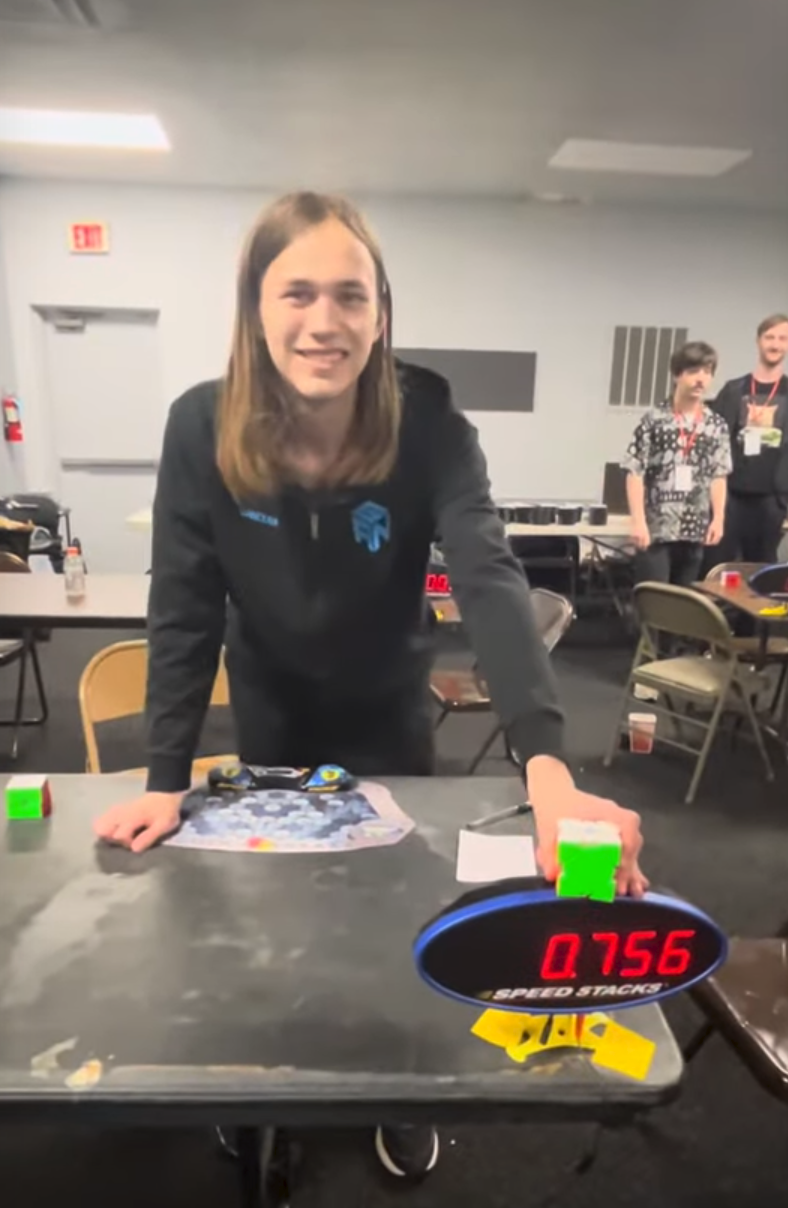
\includegraphics[width=0.95\textwidth]{carter.png}
    \end{center}
\end{column}


\begin{column}{0.8\textwidth}
 \begin{table}
    \centering
    \begin{tabular}{|c|c|c|P{2.5cm}|}
        \hline
        Solve & Result & Scramble (11 moves) & Fewest number of moves \\
        \hline
        1 & 2.49 & R B L' U' L' R B' R' B R B & 9 \\
        \hline
        2 & 1.77 & U L U' B' U' B' U' L B U' R' & 9 \\
        \hline
        3 & 3.32 & U L B U' B' L' B R' B' L U & 7 \\
        \hline
        4 & 4.65 & R B' U' B U B L' U B' U R & 8 \\
        \hline
        5 & 0.75 (WR!) & B L R' B' L U B' R U' R U & 8 \\
        \hline
    \end{tabular}
\end{table}
\end{column}
\end{columns}
\vspace{0.7cm}
\begin{itemize}
    \item The third fastest solve (0.85) was done by Simon Kellum in this competition, solving the same scramble!
\end{itemize}
\end{frame}





\begin{frame}
\frametitle{The End}
\begin{alertblock}{\centering Thank}
\centering you
\end{alertblock}
\begin{block}{\centering More details}
\centering
If you are really interested, you are welcome to ask for the code.
\end{block}
\begin{block}{\centering Download this PDF}
\centering

\includegraphics[width=0.2\textwidth]{download.png}
\end{block}
\end{frame}





\end{document}